


\usepackage[pages=some]{background}

\backgroundsetup{
scale=1,
color=black,
opacity=1,
angle=0,
contents={%
  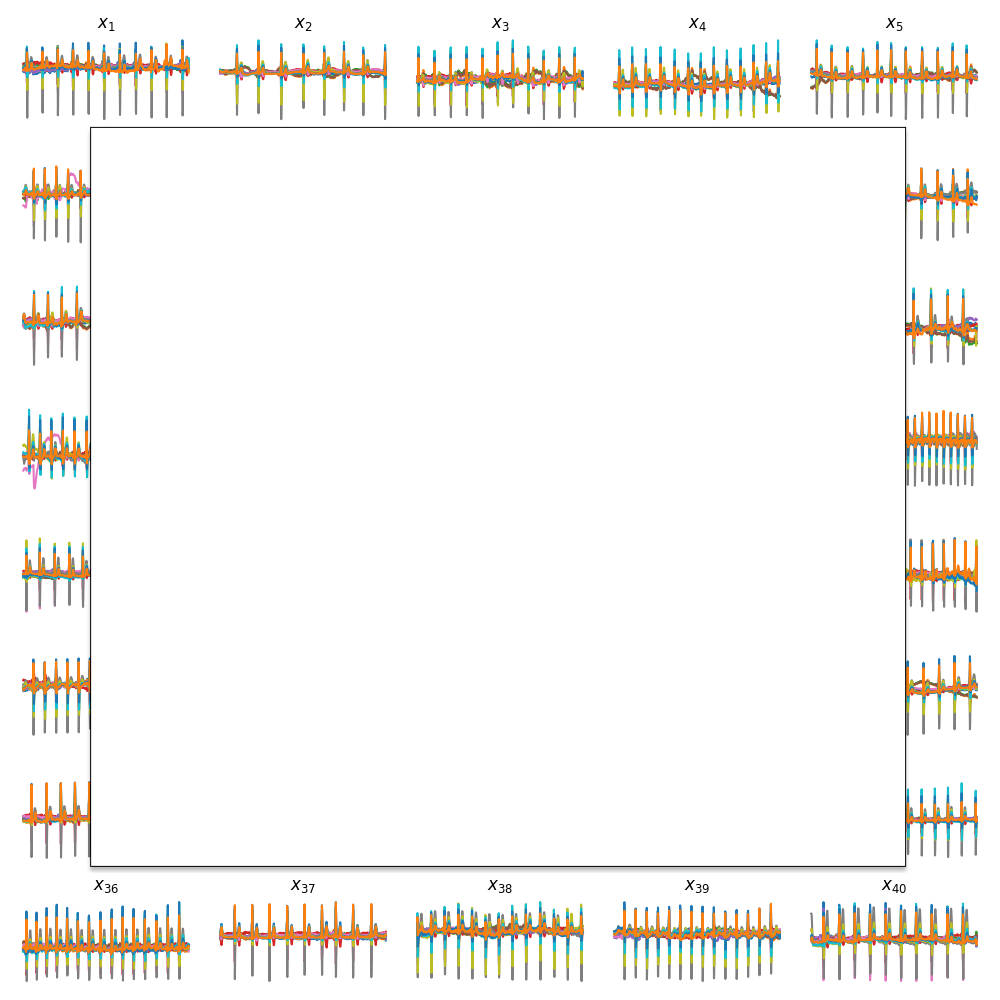
\includegraphics[width=\paperwidth,height=\paperheight]{code/results/frontpage.png}
  }%
}




%\usepackage{algorithm}
%\usepackage{algpseudocode}
\usepackage[linesnumbered, ruled]{algorithm2e}

% coloring text
\usepackage{xcolor}

% using the comment environment
\usepackage{comment}

% FOR REFERENCES
\usepackage{biblatex}
\addbibresource{references.bib}


% definitions
\usepackage{amsthm}
\usepackage{amsmath}
\usepackage{amsfonts}
\theoremstyle{remark}
\newtheorem{definition}{Definition}[section]


% links
\usepackage{hyperref}
